\documentclass[12pt, a4paper]{article}
\usepackage{titlesec}
\setcounter{secnumdepth}{4}
\usepackage[utf8]{inputenc}
\usepackage{fancyhdr}
\newcommand{\etal}{\textit{et al.}}
\usepackage{hyperref}
\usepackage{listings}
\usepackage{geometry}
\usepackage{graphicx}
\usepackage{longtable}
\usepackage[]{algorithm2e}
\usepackage{pgfplots}
\graphicspath{ {./images/} }
 \geometry{
 a4paper,
 total={170mm,257mm},
 left=20mm,
 top=20mm,
 }

\title{%
 \LARGE        CS F402 Computational Geometry
\newline
\newline
\LARGE Programming Project\\
\Large Euclidean K-Supplier Problem
}

\author{%
 \begin{tabular}{c} \small Raj Kashyap\\ \small Mallala\\ \small2017A7PS0025H \end{tabular}\and
 \begin{tabular}{c} \small L Srihari\\ \small2017A7PS1670H \end{tabular}\and
 \begin{tabular}{c}\small T Naga Sai\\ \small Bharath\\ \small2017A7PS0209H \end{tabular}
}
\date{June 2020}

\begin{document}
\maketitle
\section{Problem Statement}
Given a set \textbf{\textit{F}} of \textbf{\textit{m}} points and another set \textbf{\textit{C}} of \textbf{\textit{n}} points in the plane, the objective is to open a set $\textbf{\textit{F}}’$ $\subseteq$ \textbf{\textit{F}} of \textbf{\textit{k}} facilities such that the maximum distance of any client in \textbf{\textit{C}} to its nearest open facility in \textbf{\textit{F}}’ is minimized. The distances between the points satisfy two properties: symmetry (i.e. d(u,v) = d(v,u) for all $u,v \in \textbf{\textit{F}} \cup \textbf{\textit{C}}$) and triangle inequality (i.e $d(u,v)+d(v,w) \geq d(u,w)$ for all $u,v,w  \in \textbf{\textit{F}} \cup \textbf{\textit{C}}$).\\

Let $d(f,\textbf{\textit{F}}’)$ = minimum distance from point f to g where g is any point in  \textbf{\textit{F}}'. Then,
\begin{equation} d(f,\textbf{\textit{F}}’) = \emph{min}\;d(f,g) : g \in \textbf{\textit{F}}’\end{equation}
The given problem can be expressed as,\begin{center}\textbf{minimize} $max\;d(f,$\textbf{\textit{F}}’$)$, where\end{center}
$\;$\textit{f} $\in$  \textbf{\textit{C}} and $\textbf{\textit{F}}'$ $\subseteq$ \textbf{\textit{F}} such that $| \textbf{\textit{F}}' | = \textbf{\textit{k}}$\\

\section{Introduction}
Multiple applications of the euclidean K-supplier problem can be found. One obvious application is in the domain of facility location in supply - chain markets and businesses, commonly observed in large supermarket chains. Here the consumer outlets form the set \textbf{\textit{C}} and locations of potential intermediate suppliers form the set  \textbf{\textit{F}}.\\
Other applications include opening hospitals in a city with limited capacities, opening of centres for the disposal of obnoxious substances, setting up servers in a network, data mining and information retrieval such as data clustering.\\

\section{About the paper in concern}
The implementation for the Euclidean K Supplier problem done in this project is based on the research paper by Nagarajan \etal \cite{EuclideanKS}. They present a 2.73 approximation algorithm. It is very close to the nearest possible approximation algorithm (It is NP-hard to approximate the algorithm better than 2.65). The approach taken in this algorithm is also impressive. They use information on the pairs of clients to solve the problem. We have implemented the algorithm for 2 dimensional case.\\

\subsection{Algorithm}
As common in many bottleneck optimization algorithms, an additional parameter \textit{L} is selected ( which is the objective value ) and outputs one of the following :\\
 1. a certicate showing that the optimal k-supplier value is more than \textit{L}, or \\
 2. a k-supplier solution of value at most $\alpha$ * $\textit{L}$. where $ \alpha = 1+\sqrt(3)$ is the approximation ratio. \\
The final algorithm uses binary search to find the best value of \textit{L}. \\
 
So, for a chosen \textit{L}, we do the following. \\ 
A maximal subset of clients is selected such that the distance between any pair of clients is greater than $\sqrt(3)$ * \textit{L}. We construct a graph based on these selected clients as vertices. We also select a subset of facilities such that there is a one to one correspondence between these facilities and edges in the graph. The facilities in this subset are selected such that there is atleast one and atmost two clients in the graph within distance \textit{L}.\\
In other words, there is an edge for a pair of vertices in that graph, if there is a facility which is at distance less than \textit{L} from both the vertices. For a client, if there is no such partner client satisfying that rule, then there is a self loop for that client in the graph. \\
More formally, lets say the new graph \textit{G} has the vertex set \textit{P} edge set \textit{E}=\textit{E1} $\cup$ \textit{E2} \\
  \textit{E1} = {(\textit{u,v}) : $\textit{u,v} \in \textit{P}$, $\exists\textit{f} \in \textit{F}$ with $\textit{d(u,f)} \leq \textit{L}$ and $\textit{d(v,f)} \leq \textit{L}$} \\
 \textit{E2} = {(\textit{u,u}) : $\textit{u} \in \textit{P}$, $\exists\textit{f} \in \textit{F}$ with $\textit{d(u,f)} \leq \textit{L}$ and $\forall \textit{v} \in \textit{P}$, $\textit{(u,v)} \notin \textit{E1}$} \\
Then we find the minimum edge cover on this new graph \textit{G}. If the number of edges in the minimum edge cover is greater than \textit{k}, then the optimal value is greater than \textit{L} else output the facilities corresponding to the edges in the minimum edge cover. \\
 
For constructing the graph, we have used an algorithm for finding the approximate nearest neighbour with $(1+\epsilon)$ approximation ratio $(\epsilon=0.2)$ by Arya and Mount.\\
And also, for finding minimum edge cover, we find the maximum matching of \textit{G} using Micali and Vazirani's algorithm and then in linear time find the minimum edge cover of \textit{G} \\

  
 \subsection{Time Complexity}
Generally for constructing the graph, it takes $O(n^2)$ time which involves finding the vertices and then edges. But using approximate nearest neighbours algorithm by Arya and Mount, we can construct the graph in $O(nlog{}n)$ time complexity but with a loss of $1+\epsilon$ factor.
And the fastest known edge cover algorithm is finding the maximum matching and in linear time find the minimum edge cover. Micali and Vazirani's maximum matching algorithm runs in $O(\textit{E $\sqrt{V}$})$. In our case, $\textit{E} \leq \textit{n}$ and $\textit{V} \leq \textit{n}$. Because every edge has a corresponding facility and therefore edges are less than number of facilities. And also, the number of vertices is a subset of clents and therefore number of vertices is less than total number of clients. Here, \textit{n} is number of facilities and clients combined. Therefore, this step takes $O(n^{1.5})$ time. \\
For finding the minimum edge cover from maximum matching takes linear time. Because we go through the graph once and note the unsaturated vertices (vertices which don't have any edge in maximum matching). Now for every such vertex, we add any of the edge of that vertex to the set of maximum matched edges. In this way, every vertex is covered and we have minimum edge cover. \\
Considering both the steps of creating the graph and finding the minimum edge cover on it, our algorithm runs in $O(n^{1.5})$ time.



\subsection{Pseudocodes and Explanation}
\begin{algorithm}[H]
 Pick a maximal subset $P \subset C$ such that each pairwise distance in P is more than $\sqrt{3}.L$\;
 Construct graph G=(P,E) with vertex set P and edge set $E = E1 \cup E2$, where \newline
 E1 =  {(u,u) : $ u \in P, \exists f \in F $ with $d(u,f) \leq L$ and $d(v,f) > L \forall v \in P\backslash u$}\;
 E2 =  {(u,v) : $u,v \in P, \exists f \in F$ with $d(u,f) \leq L$ and $d(v,f) \leq L$}\;
 Compute the minimum edge cover $T \subset E$ in G\;
 \eIf{$|T| > k$}{
 the optimal value is larger than L\;
 }{output the facilities corresponding to T as solution\;}
 \caption{Algorithm for Euclidean k-supplier\newline}
 \end{algorithm}

As a part of this algorithm, we are required to calculate the minimum edge cover. We achieve this by first finding the set of edges in the maximum match and then for each vertex of degree zero, add any of its edges to the set. It can be shown that this effectively converts the output of maximum matching algorithm (\cite{MicaliVazirani}) to a set of edges in minimum edge cover, as required by the Euclidean k-Supplier algorithm.\\

\begin{algorithm}[H]
$M \gets$ output of Maximum Matching on Auxillary graph\;
 \For{each vertex v of degree 0}{
 Pick any edge e connected to v\;
 Add e to M\;
 }
 Output M\;
 \caption{Minimum edge cover from Maximum Matching\newline}
 \end{algorithm}
\begin{algorithm}[H]
 $P \gets \emptyset$ and $ P' \gets \emptyset$ \;
 \For{$v \in C$}{
  $v' \gets $ approximate nearest neighbor of v in P'\;
  \If{$d(v,v')>\sqrt{3}(1+\epsilon)^2\textit{L}$ or v' = NIL}{
  $P \gets P \cup{v}$ and insert v into P'\;
   }
 }
\caption{Algorithm for computing vertices\newline\newline}
\end{algorithm}

\begin{algorithm}[H]
 Construct data structure P' containing points P, and initialize $E \gets \emptyset$\;
 \For{$f \in F$}{
  $u \gets$ approximate nearest neighbor of f in P'\;
  $v \gets$ approximate second nearest neighbor of f in P'\;
  \If{$d(u,f)\leq(1+\epsilon)\textit{L}$ and $d(v,f) > (1+\epsilon)\textit{L}$}{
   set $E \gets E \cup {(u,u)}$ and label edge (u,u) by facility f.\;
   }
   \If{$d(u,f)\leq(1+\epsilon)\textit{L}$ and $d(v,f) \leq (1+\epsilon)\textit{L}$}{
   set $E \gets E \cup {(u,v)}$ and label edge (u,v) by facility f.\;
   }
 }
 Output E\;
 \caption{Algorithm for computing Edges\newline\newline}
\end{algorithm}

\section{Results}
The $(1+\sqrt{3})$ approximation Euclidean k-Supplier algorithm proposed in \cite{EuclideanKS} has two major sub-routines, namely, An algorithm for finding maximum matching in general graphs \cite{MicaliVazirani} and An optimal algorithm for approximate nearest neighbor searching in fixed dimensions  (Sunil Arya and David M. Mount \cite{ANN}), which are by themselves well researched in the algorithmic domain. In this programming assignment, the first major subroutine on Maximum Matching, also known as the MV algorithm, has been programmed from the scratch based on the algorithmic exposition given by Paul A. Peterson and Michael C. Loui \cite{Exposition}. The second major subroutine on Approximate nearest neighbors has been implemented with the aid of the ANN library provided for public use by the authors themselves \cite{ANNLibrary}. The complete coding was done in C plus plus programming language. As the performance and correctness of the subroutines are crucial for efficient working of the main algorithm, we provide the results of unit tests on these sub routines first. The unit tests are followed by results of the complete algorithm.\\
\subsection{Unit test on component Algorithms}
Unit tests for Maximum Matching algorithm was conducted with input from NetworkX python library. The library's builtin max\_weight\_matching method was used to test the results of our code. It was observed that the number of matchings were same for all 36 unit tests conducted. The running time of our algorithm was found to be faster for large size of input graphs. 16 of the different varieties of unit tests have been tabulated in the table 4.1. The choice of unit tests were based on the variety in the type of graph for the first 11 tabulated entries and the remaining were tested for large size of input. The input and output corresponding to each of these entries have been documented in an accompanying text file.\\
Since, the nearest neighbors identified by \cite{ANN} are not easily verifyable because of their approximate nature (there is no single correct answer in many cases), we refrain from testing the algorithm for its correctness. Also, since the implementation has been taken from a public and well documented library, it is expected that the correctness would have been established by the authors themselves. Further, this algorithm is based on the research paper \cite{ANN} as ground truth, hence the algorithm's time complexity need not be tested because of the fact that the library was created to perform with the proven $O(n^2)$ worst case complexity and $O(log^3 n)$ expected time. The following subsection provides the unit tests on the maximum matching implementation by us.

\subsubsection{Maximum Matching Algorithm (MicaliVazirani.cpp)}
{\renewcommand{\arraystretch}{2}
\begin{longtable}{ |p{2cm}||p{2cm}|p{2cm}|p{2cm}|p{2cm}| p{2cm}|  }
 \hline
 \multicolumn{6}{|c|}{Unit test results} \\
 \hline
Type of graph & Number of nodes &Number of edges & Running Time (microseconds) & Size of NetworkX output & Size of our output\\
 \hline
Single Bloom, Two extensions   & 7   &7& 996&3&3  \\\hline
Two Blooms, Three connecting edges   & 12   &13& 990&6&6  \\\hline
Two blooms, three connected components   & 10   &15& 995&5&5  \\\hline
Two blooms, one embedded inside other   & 9   &11& 997&4&4  \\\hline
Two blooms, one embedded , connected at centre &9&11&999&4&4 \\\hline
Three blooms, three connections   & 16   &18& 997&7&7  \\\hline
Three hexagons, three bridges, Two extensions   &19  &21& 974&9&9  \\\hline
Peterson graph & 10  &15& 309&5&5  \\\hline
Bull graph   & 5   &5& 1019&2&2  \\\hline
Dodecahedral graph   &20  &30 & 944 &10&10  \\\hline
Frucht graph   &12   &18 & 997 &6&6  \\\hline
Medium size 2D graph   & 100   &180& 5018&50&50  \\\hline
Medium barbell graph   & 30   &101& 1995&15&15  \\\hline
Large Barbell graph   &121   &2472& 42883&60&60  \\\hline
Large ladder graph   & 2000   &2998& 80748&1000&1000  \\\hline
Large Erdos Renyi Random graph &500 &74716& 1056175&250&250 \\\hline

 \hline
\end{longtable}

\subsection{Results of the main algorithm}
\begin{longtable}{ |p{2cm}|p{2cm}|p{2cm}|p{2cm}|p{2cm}| p{2cm}|  }
 \hline
 \multicolumn{6}{|c|}{Unit test results} \\
 \hline
Type of graph & k- value & Number of Client nodes &Number of Facility nodes & Running Time (microseconds) & Best L value\\
 \hline
Single Bloom, Two extensions   & 7   &7& 996&3&3  \\\hline
Two Blooms, Three connecting edges   & 12   &13& 990&6&6  \\\hline
Two blooms, three connected components   & 10   &15& 995&5&5  \\\hline
Two blooms, one embedded inside other   & 9   &11& 997&4&4  \\\hline
Large grid of clients and few facilities &2&10000&11&1320631&35.0703 \\\hline
Rainbow arc of client and facilities   & 3  &75& 14&13146&2.53125  \\\hline
Alternate rainbows of client and facilities&10 &27 &21&26934&1.09659  \\\hline
Peterson graph & 10  &15& 309&5&5  \\\hline
Bull graph   & 5   &5& 1019&2&2  \\\hline
Dodecahedral graph   &20  &30 & 944 &10&10  \\\hline

 \hline
\end{longtable}

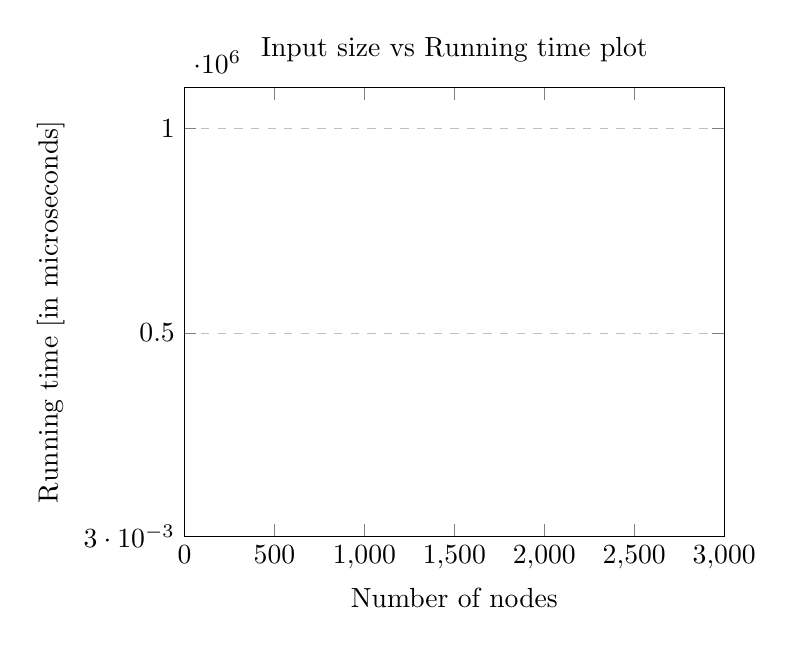
\begin{tikzpicture}
\begin{axis}[
    title={Input size vs Running time plot},
    xlabel={Number of nodes},
    ylabel={Running time [in microseconds]},
    xmin=0, xmax=3000,
    ymin=3000, ymax=1100000,
    xtick={0,500,1000,1500,2000,2500,3000},
    ytick={3000, 500000, 1000000},
    legend pos=north west,
    ymajorgrids=true,
    grid style=dashed,
]

\addplot[
    color=blue,
    mark=square,
    ]
    coordinates {
    };
    \legend{}
    
\end{axis}
\end{tikzpicture}

\section{Conclusions from the empirical study}

\section{Appendix: Type of input and expected output for each enclosed cpp file}
\subsection{MicaliVazirani.h}
\textbf{Input}: An object of the class MicaliVazirani must be instantiated by passing an adjacency list in the form of $map< int, vector<int>>$ to the construtor. Then the method general\_matching\_algorithm can be called on that object.\\

\textbf{Output}: The function general\_matching\_algorithm returns a $map<pair<int,int>,pair<int,int>>$. If the input had was of single dimension then the second element of pair is taken as `0'.

\subsection{euclideanKSupplier.cpp}
\textbf{Environment variables for ANN}: \\CPLUS\_LIBRARY\_PATH = $<$path to include files$>$\\
LIBRARY\_PATH = $<$path to library containing .a files in Linux or .DLL and .lib in Windows$>$\\

\textbf{Compilation}: g++ euclideanKSupplier.cpp -lANN\\

\textbf{Input}: Input is through command line.\\
./a.out (k) (clients file) (facilities file) [in Linux]\\
./a.exe (k) (clients file) (facilities file) [in Windows]\\

\textbf{Output}: The best possible L value and the facilities corresponding to that value of L\\

\begin{thebibliography}{5}
\bibitem{EuclideanKS} 
Viswanath Nagarajan, Baruch Schieber, and Hadas Shachnai
\textit{The Euclidean k-Supplier Problem}.
Integer Programming and Combinatorial Optimization. IPCO 2013.

\bibitem{MicaliVazirani} 
 Silvio Micali, Vijay V. Vazirani
\textit{An algorithm for finding maximum matching in general graphs}.
21st Annual Symposium on Foundations of Computer Science (sfcs 1980)

\bibitem{Exposition} 
Paul A. Peterson, Michael C. Loui
\textit{The general maximum matching algorithm of micali and vazirani}.
Algorithmica 3, 511–533 (1988). https://doi.org/10.1007/BF01762129

\bibitem{ANN} 
Sunil Arya, David M. Mount
\textit{Approximate nearest neighbor queries in fixed dimensions}.
SODA '93: Proceedings of the fourth annual ACM-SIAM symposium on Discrete algorithms, January 1993

\bibitem{ANNLibrary} 
Sunil Arya, David M. Mount
\textit{ANN: A Library for Approximate Nearest Neighbor Searching}.
http://www.cs.umd.edu/~mount/ANN/
\end{thebibliography}
\end{document}